\chapter{Introducción}

Hoy en día es habitual que los datos que usamos estén almacenados en una Base de Datos. Da igual que ese dato lo estemos utilizando desde un navegador web, en una aplicación de móvil o una videojuego. Cada consulta que realicemos al dato y cada posible modificación o eliminación del mismo realizará una petición (consulta o modificación) a un Sistema Gestor de Base de Datos.

Cada consulta realizada, cada petición de actualización o cada eliminación de datos, tendrá que ser procesada por el Gestor de Base de Datos y analizada para comprobar que lo que se va a realizar, como los permisos de quién pide la acción son adecuados, para posteriormente realizar la acción.

Los datos almacenados en una base de datos son de gran importancia en una empresa, por lo que la continuidad del servicio, así como la seguridad de los accesos recae en los administradores de Bases de Datos (DBA o DataBase Administrator) que deberán asegurar que el funcionamiento sea el esperado, así como la gestión de copias de seguridad de los mismos.

A lo largo de esta asignatura recordaremos los conceptos básicos de las bases de datos, comprenderemos la importancia y las funciones que desempeñan un Sistema Gestor de Base de Datos, aprenderemos a administrar el SGBD, crear y gestionar backups así como montar un sistema en \hyperlink{altadisponibilidad}{Alta Disponibilidad}.

\chapter{Repaso}
A modo de repaso rápido de la asignatura Gestión de Bases de Datos, veremos rápidamente unos conceptos que nos deberían ser conocidos.


\section{¿Qué es una Base de Datos?}
Recordemos que una base de datos es un conjunto de datos que suelen pertenecer a un mismo contexto y que está almacenado para poder ser consultado posteriormente. Aunque actualmente una base de datos se asocia a un sistema informático, una biblioteca también puede considerarse una base de datos, ya que almacena libros que se pueden consultar, y el bibliotecario (el que te da acceso a los libros, si es que perteneces a la biblioteca) podría ser el símil del sistema gestor de la base de datos.

Actualmente las bases de datos se encuentran en todos los lugares, no sólo en servidores específicamente creados para ellos. Algunos ejemplos:

\begin{itemize}
    \item Cada vez que usamos una aplicación de móvil, la propia aplicación cuenta con una base de datos interna (aparte de los datos que pueda consultar a bases de datos externas)
    \item Las páginas web que visitamos almacenan datos en pequeñas bases de datos en los propios navegadores que usamos.
    \item Aplicaciones de escritorio que guardan las preferencias del usuario en bases de datos.
\end{itemize}


No todas las bases de datos tienen por qué ser gestionadas por sistemas gestores (como los ejemplos puestos previamente), ya que el acceso a los datos quizá no sea necesario que esté controlado, pero en entornos empresariales es lo habitual.

\section{Tipos de Bases de Datos}
Las bases de datos se pueden clasificar de varias maneras, teniendo en cuenta el contexto que estemos manejando, las necesidades que tengamos, el tipo de datos que estemos utilizando…

Nos vamos a centrar en la clasificación teniendo en cuenta los distintos modelos de administración de los datos, concrétamente en el \textbf{modelo relacional}, aunque veremos otros también utilizados.


\subsection{Bases de datos relacionales}
Es el modelo más utilizado actualmente para representar problemas reales y administrarlos de manera dinámica. El paradigma nació en \textbf{1970} de la mano de \href{https://es.wikipedia.org/wiki/Edgar_Frank_Codd}{Edgar Frank Codd} cuya idea es el uso de “relaciones”.

\begin{wrapfigure}{r}{0.36\linewidth}
    \centering
    \vspace{-15pt}
    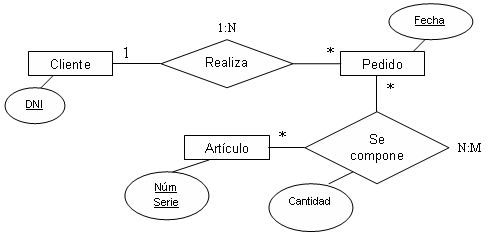
\includegraphics[width=\linewidth]{ejemplo_diagrama_E-R_extendido.png}
    \vspace{-30pt}
    \captionof{figure}{\href{https://commons.wikimedia.org/wiki/File:Ejemplo_Diagrama_E-R_extendido.PNG}{Origen: Wikipedia}}
    \vspace{-30pt}
\end{wrapfigure}
En este modelo, el lugar y la forma en que se almacenen los datos no tienen relevancia (que sí tenían otros modelos previos).

Para que una base de datos sea considerada relacional debe de seguir el modelo relacional, por lo que antes de introducir datos, para crear la base de datos \textbf{habremos realizado los pasos necesarios para pasar del modelo entidad-relación al modelo relacional}. Es por ello que hay que acordarse siempre de realizar la \textbf{normalización de la base datos}.

Para este tipo de bases de datos el lenguaje de consultas utilizado es el \textbf{SQL} (en inglés \textit{Structured Query Language}; en castellano: lenguaje de consulta estructurada) el cual abordaremos más adelante.


\subsection{No relacionales}
Antes y después de la aparición del modelo relacional han existido distintos modelos de base de datos (jerárquico, de red, multidimensionales… ), por lo que hay que entender que el relacional no es el único modelo existente, aunque sí el más utilizado.


\subsubsection{Bases de datos Documentales}
Las bases de datos documentales son aquellas que se encargan de almacenar datos de tipo documento, también conocidos como datos semi-estructurados.

En el dato almacenado puede existir una estructura fija, o que puede ser modificada en el tiempo. Normalmente esta información suele estar almacenada en \hyperlink{json}{JSON} o XML.

Este tipo de bases de datos entran dentro de las denominadas \href{https://es.wikipedia.org/wiki/NoSQL}{NoSQL}, cuyos datos no requieren estructuras fijas como tablas y cuyo acceso suele realizarse mediante el sistema “clave-valor”.

Las bases de datos NoSQL están altamente optimizadas para las operaciones recuperar y agregar, y normalmente no ofrecen mucho más que la funcionalidad de almacenar los registros. No suele ser habitual el poder realizar consultas de tipo JOIN, por lo que este tipo de operaciones se realizaría desde la aplicación que realiza las consultas de obtención de datos.

No entraremos en este modelo de base de datos, debido a sus diferencias con el modelo relacional, pero es obligatorio conocer que existen y que son utilizadas en aplicaciones como las redes sociales (por ejemplo).

Algunos ejemplos de gestores NoSQL son: \href{https://es.wikipedia.org/wiki/MongoDB}{MongoDB}, \href{https://es.wikipedia.org/wiki/Elasticsearch}{Elasticsearch}, …


\chapter{Sistemas Gestores de Bases de Datos}
\begin{wrapfigure}{r}{0.17\linewidth}
    \centering
    \vspace{-20pt}
    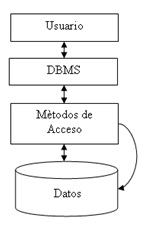
\includegraphics[width=\linewidth]{Componentes_de_un_base_de_datos.jpg}
    \vspace{-33pt}
    \captionof{figure}{\href{https://commons.wikimedia.org/wiki/File:Componentes_de_un_base_de_datos.jpg}{Origen: Wikipedia}}
    \vspace{-30pt}
\end{wrapfigure}
Un Sistema Gestor de Base de Datos es un conjunto de programas que permiten el almacenamiento, modificación y consulta de datos de una base de datos. Teniendo en cuenta los permisos del solicitante se le otorgarán ciertos privilegios lo que hará que se le permitirá acceder (o no) a ciertas funciones que podrá realizar sobre los datos.

Estos sistemas proporcionan distintas tareas para mantener la integridad de los datos, administrar el acceso y la opción de recuperar información en caso de que el sistema se corrompa.

Tal como se puede ver en la imagen, el ejemplo de uso habitual de un Sistema Gestor de Base de Datos se puede resumir de la siguiente forma:

\begin{itemize}
    \item El usuario se comunica con el SGBD (Sistema Gestor de Base de Datos, o en inglés DBMS: DataBase Management System).
    \item El SGBD comprueba que el usuario tiene permisos para acceder a los datos.
    \item El SGBD conoce cómo están almacenados los datos por lo que hará uso del método de acceso adecuado de cómo se han guardado los datos.
    \item Se recuperan los datos del dispositivo físico concreto donde estén almacenados los datos, teniendo en cuenta los datos pedidos por el usuario y el método de acceso.
    \item Se le entregan los datos al usuario.
\end{itemize}

Todas estas tareas deben de realizarse de la manera más rápida posible, por lo que la optimización de cada una de las partes debe de ser adecuada.


\section{Componentes de un SGBD}
Normalmente un SGBD tiene los siguientes componentes:

\begin{itemize}
    \item El \textbf{motor de la base de datos} acepta peticiones lógicas de los otros subsistemas del SGBD, las convierte en su equivalente físico y accede a la base de datos y diccionario de datos en el dispositivo de almacenamiento.
    \item El \textbf{subsistema de definición de datos} ayuda a crear y mantener el diccionario de datos y define la estructura del fichero que soporta la base de datos.
    \item El \textbf{subsistema de manipulación} de datos ayuda al usuario a añadir, cambiar y borrar información de la base de datos y la consulta para extraer información. El subsistema de manipulación de datos suele ser la interfaz principal del usuario con la base de datos, y normalmente se hace uso del lenguaje SQL.
    \item El \textbf{subsistema de administración} ayuda a gestionar la base de datos ofreciendo funcionalidades como almacenamiento y recuperación, gestión de la seguridad, optimización de preguntas, control de concurrencia y gestión de cambios.
\end{itemize}

Dependiendo del SGBD que utilicemos, podremos contar con otros apartados que vienen incluídos, o programas externos que podremos utilizar para ampliar alguna funcionalidad del mismo.

\section{Modelo ACID de transacciones}
En bases de datos se denomina \textbf{ACID} a las características de los parámetros que permiten clasificar las transacciones de los sistemas de gestión de bases de datos, donde ACID es un acrónimo en inglés de \textit{\textbf{A}tomicity, \textbf{C}onsistency, \textbf{I}solation and \textbf{D}urability} (en castellano: Atomicidad, Consistencia, Aislamiento y Durabilidad).

Las definiciones son:

\begin{itemize}
    \item \textbf{Atomicidad}: Una transacción es una unidad lógica de trabajo que contiene una o varias sentencias SQL. El principio básico de una transacción es el todo o nada, una operación atómica tiene éxito o falla como un todo.
        \begin{itemize}
            \item Un SGBD ha de ser capaz de asegurar la integridad de los datos ante la concurrencia de varios usuarios a la vez.
            \item Un SGBD debe de ser capaz de agrupar varias sentencias SQL,de tal manera que puedan ser validadas (\textbf{commit}) o desechadas (\textbf{rollback}) como una unidad.
            \item \textbf{Ejemplo}: en el caso de una transacción bancaria o se ejecuta tanto el depósito y la deducción o ninguna acción es realizada
        \end{itemize}
    \item \textbf{Consistencia}: (Integridad). Es la propiedad que asegura que sólo se empieza aquello que se puede acabar. Por lo tanto se ejecutan aquellas operaciones que no van a romper las reglas y directrices de Integridad de la base de datos.
        \begin{itemize}
            \item El SGBD debe asegurar que cualquier transacción llevará a la base de datos desde un estado válido a otro también válido.
            \item El SGBD debe asegurar que los datos son exactos y consistentes, es decir que estén siempre intactos, sean siempre los esperados y que de ninguna manera cambian ni se deformen. De esta manera podemos garantizar que la información que se presenta al usuario será siempre la misma.
        \end{itemize}
    \item \textbf{Isolation / Aislamiento}: Esta propiedad asegura que una operación no puede afectar a otras.
        \begin{itemize}
            \item Esto asegura que la realización de dos transacciones sobre la misma información sean independientes y no generen ningún tipo de error.
            \item Esta propiedad define cómo y cuándo los cambios producidos por una operación se hacen visibles para las demás operaciones concurrentes.
            \item El aislamiento puede alcanzarse en distintos niveles, siendo el parámetro esencial a la hora de seleccionar SGBDs.
        \end{itemize}
    \item \textbf{Durabilidad / Persistencia}: Esta propiedad asegura que una vez realizada la operación, ésta persistirá y no se podrá deshacer aunque falle el sistema y que de esta forma los datos sobrevivan.
\end{itemize}

\section{Software SGBD}
Actualmente existen distintos SGBD que podemos instalar en nuestros servidores. Cada uno de ellos cuentan con sus características propias, por lo que tendremos que conocer las necesidades que tenemos a la hora de elegir entre ellas.

\begin{itemize}
    \item \href{https://es.wikipedia.org/wiki/MySQL}{MySQL}: base de datos relacional, desarrollada por Oracle desde que en 2008 ésta se hiciera con Sun Microsystems y de licencia libre (aunque también cuenta con una versión no-libre).
    \item \href{https://es.wikipedia.org/wiki/PostgreSQL}{PostgreSQL}: base de datos relacional, desarrollada por PostgreSQL Global Development Group y de licencia libre.
    \item \href{https://es.wikipedia.org/wiki/Microsoft_SQL_Server}{SQL Server}: base de datos relacional, desarrollada por Microsoft.
    \item \href{https://es.wikipedia.org/wiki/Oracle_Database}{Oracle Database}: base de datos de tipo objeto-relacional desarrollada por Oracle Corporation.
    \item \href{https://en.wikipedia.org/wiki/IBM_Db2_Family}{DB2}: base de datos relacional, desarrollada por IBM.
    \item \href{https://es.wikipedia.org/wiki/MongoDB}{MongoDB}: base de datos documental, desarrollada por MongoDB y de licencia libre.
    \item \href{https://es.wikipedia.org/wiki/Apache_Cassandra}{Cassandra}: base de datos NoSQL distribuida y basada en el modelo clave-valor, desarrollada por Apache y de licencia libre.
    \item \href{https://es.wikipedia.org/wiki/Elasticsearch}{Elasticsearch}: base de datos documental que cuenta con un servidor de búsqueda de texto completo.
\end{itemize}

Existen otros SGBD (tanto relacionales como no), pero el listado muestra las más conocidas y utilizadas a día de hoy. La elección del SGBD que vayamos a utilizar en nuestro proyecto debería ir acompañado de un análisis profundo de las características de cada uno de ellos, así como de las necesidades que requerimos.


\chapter{MySQL como Sistema Gestor de Base de Datos}
\begin{wrapfigure}{r}{0.25\linewidth}
    \centering
    \vspace{-20pt}
    
\includegraphics[width=\linewidth]{MySQL_logo.png}
    \vspace{-60pt}
\end{wrapfigure}
El SGBD que usaremos durante esta asignatura es MySQL.


\section{Introducción}
MySQL es un sistema de gestión de bases de datos relacional desarrollado actualmente por Oracle Corporation, conocida empresa que también tiene su sistema SGBD Oracle privativo. MySQL cuenta con una \textbf{licencia dual}: Licencia Pública General (\hyperlink{licencias_libres}{GPL}) y licencia comercial, por lo que en su página web podremos encontrar ambas versiones (la primera de código abierto y gratuita, y la segunda con opción de pago, con servicios extra  y soporte).

Actualmente MySQL está considerada como la base de datos relacional de código abierto más popular y se puede instalar en los tres sistemas operativos más conocidos actualmente.


\subsection{Un poco de historia}
MySQL fue inicialmente desarrollado por MySQL AB (empresa fundada por David Axmark, Allan Larsson y Michael Widenius). MySQL AB fue adquirida por Sun Microsystems en 2008, y ésta a su vez fue comprada por Oracle Corporation en 2010.

Es cierto que aunque en sus primeras versiones carecía de características como la integridad referencial y transacciones (debido al motor MyISAM utilizado en la creación de tablas), que son características muy importantes en un SGBD (y que \href{https://es.wikipedia.org/wiki/PostgreSQL}{PostgreSQL} sí tenía), no impidió que cogiera fama en los denominados entornos LAMP (Linux + Apache + MySQL + PHP).

Poco antes de la compra de Oracle, desde la comunidad libre se realizó un fork (una copia completa) del código fuente de MySQL que dió origen a \textbf{MariaDB}. Desde ese momento, ambos SGBD han tenido vidas paralelas, pero el origen es el mismo.

Muchas distribuciones GNU/Linux contaban con MySQL como sistema SGBD para poder ser instalado, pero a medida que el desarrollo de MariaDB fue ganando adeptos muchas distribuciones realizaron el cambio, por lo que en ciertas distribuciones no es posible instalar MySQL desde los \hyperlink{repositorio_de_software}{repositorios oficiales}. De hecho, algunas distribuciones mantienen el \hyperlink{paquete_de_software}{paquete} MySQL pero siendo un alias para que se instale MariaDB.

Desde la compañía \href{https://www.percona.com/}{Percona} también crearon un fork de MySQL en el que añaden mejoras creadas por ellos y también venden soporte para el mismo.

Como veremos a continuación, el no poder realizar la instalación desde los repositorios oficiales no nos impedirá tener MySQL instalado en nuestro sistema.


\subsection{Versiones de MySQL}
MySQL cuenta con distintas versiones de SGBDs que hay que conocer para saber qué versión se necesita en cada caso concreto. Nos vamos a centrar en las versiones \textbf{Community} (las de licenciamiento libre), pero estas versiones también cuentan con su versión con licencia comercial.

\subsubsection{MySQL Community Server}
Es el SGBD que vamos a utilizar. Es la versión “clásica” de MySQL como SGBD, que permite crear bases de datos, introducir datos, manipularlos, … Esta versión cuenta con la opción de crear un sistema replicado “Primario → Réplica” o “Primario ←→ Primario” como veremos a lo largo del curso.

\subsubsection{MySQL Cluster}
Originalmente MySQL no soportaba crear clusters de servidores, sólo el sistema de replicación que soporta la versión “Community Server”, por lo que surgió la necesidad de poder crear un sistema clusterizado de 3 nodos o más que se gestionasen entre ellos, mantuvieran la información replicada… Eso se pudo realizar gracias a la librería Galera, que sirve para sincronizar la replicación de múltiples padres.

Hay que recordar que \textbf{MySQL Server es distinto a MySQL Cluster}, aunque desde un punto de vista de usuario que no entiende pueda parecer lo mismo.

\subsubsection{MySQL Router}
MySQL Router provee un enrutado transparente entre la aplicación de un usuario y cualquier servidor de MySQL. Puede sernos útil en sistemas de alta disponibilidad o de escalado para enrutar el tráfico al backend que más nos interese.

\subsubsection{MySQL Workbench}
Es un interfaz gráfico que nos proporciona herramientas para comprobar el estado de MySQL en el sistema remoto que tengamos que administrar. Existen versiones para distintos sistemas operativos y podremos instalarlo para conectarnos a servidores MySQL Remotos.

\section{Características de MySQL Community Server}
MySQL cuenta con una serie de características que hace que sea utilizado como SGBD de manera generalizada actualmente. Entre las características a destacar:

\begin{itemize}
    \item \textbf{Facilidad de uso}: Es un SGBD sencillo de utilizar en comparación con otras alternativas libres o privativas (PostgreSQL u Oracle respectivamente)
    \item \textbf{Soporte de motores de almacenamiento}: Hasta la versión 5.5 se hacía uso del motor MyISAM que no tenía integridad referencial, pero eso se cambió por el uso del motor \textbf{InnoDB} que es el utilizado actualmente. \href{https://dev.mysql.com/doc/refman/8.0/en/storage-engines.html}{Soporta varios motores}, entre los que podemos destacar:

    \begin{itemize}
        \item \textbf{InnoDB}: el utilizado por defecto actualmente. Es ACID compliant, seguro en transacciones, posibilidad para realizar commit y rollback.
        \item \textbf{MyISAM}: debería usarse sólo para tablas de lectura, ya que no soporta transacciones, pero es muy rápido.
        \item \textbf{Memoria}: se guarda toda la información en RAM, por lo que no sirve para persistencia de datos, pero hace que la información sea más rápida al acceder a ella
        \item \textbf{CSV}: las tablas realmente son ficheros de texto en formato CSV. No soporta indexado.
    \end{itemize}

    \item \textbf{Diseño multi-thread}: por lo que permite hacer uso de múltiples hilos de CPU en caso de que estén disponibles.
    \item \textbf{Replicación}: Permite crear entornos de replicación Primario → Réplica y Primario ←→ Primario.
    \item \textbf{Multiplataforma}: Funciona en distintas plataformas (distintas versiones de GNU/Linux, MacOS, Windows, FreeBSD, …).
    \item \textbf{Software Libre}: Tiene \hyperlink{licencias_libres}{licencia libre} lo que hace que podamos ver cómo funciona, y realizar modificaciones al código. Con ello se ha conseguido:
    \begin{itemize}
        \item \textbf{Mucho soporte de la comunidad}: Existen muchas herramientas realizadas por la comunidad que facilitan el uso y/o la administración de servidores MySQL.
    \end{itemize}
\end{itemize}

\section{Instalación de MySQL Community Server}
Como ya se ha mencionado antes, en algunas distribuciones MySQL ha sido sustituido por MariaDB (como en el caso de Debian), mientras que en otras se puede realizar la instalación de cualquiera de las dos (el caso de \hyperlink{ubuntu}{Ubuntu}).

Aunque haremos uso de la distribución Ubuntu, también se va a explicar brevemente cómo se haría la instalación en sistemas donde no podemos contar con el paquete en el repositorio oficial.

\subsection{Sin paquete en el repositorio oficial}
En caso de que nuestra distribución no cuente con el paquete en los repositorios oficiales, la instalación no será tan directa, pero eso no significa que sea difícil. La versión Community Server la podremos encontrar en su \href{https://dev.mysql.com/downloads/mysql/}{web de descarga}, y desde aquí podremos descargarnos la versión que necesitemos para el sistema operativo que queramos.

En el caso de que queramos instalarlo en una distribución de GNU/Linux como Debian, Red Hat o Suse podremos hacer uso de los repositorios oficiales de MySQL para realizar la instalación. En el caso de Debian, sería:

\begin{itemize}
    \item Descargar el paquete para poder configurar el repositorio oficial de MySQL para Debian/Ubuntu.
    \item Instalar el paquete:
\begin{mycode}{Instalar paquete MySQL descargado de la web oficial}{console}{}
ruben@server1:~$ sudo dpkg -i mysql-apt-config_0.8.15-1_all.deb
\end{mycode}
    \item Elegir en el menú que nos aparecerá:
    \begin{itemize}
        \item En qué distribución estamos (ya que el mismo paquete sirve para Debian y Ubuntu).
        \begin{center}
            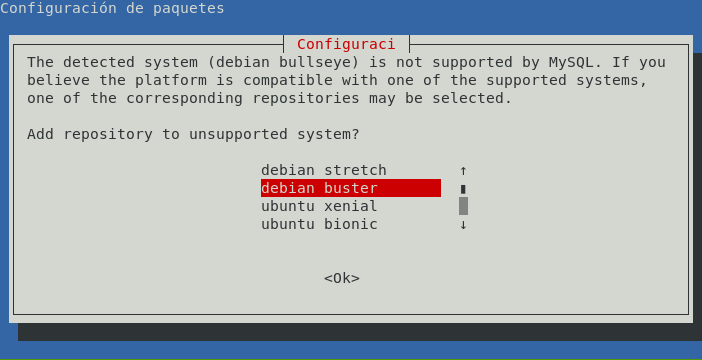
\includegraphics[width=0.6\linewidth]{install_1.png}
        \end{center}

        \item Qué versión vas a querer instalar (dependiendo de la distribución y la versión en la que nos encontremos nos dejará unas versiones u otras).
        \begin{center}
            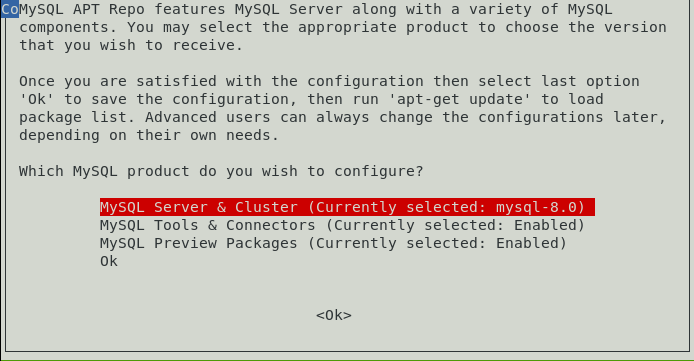
\includegraphics[width=0.6\linewidth]{install_2.png}
        \end{center}
    \end{itemize}

    \item Instalar mysql-server (tal como veremos a continuación en Ubuntu).

\end{itemize}


\subsection{En Ubuntu 20.04}
La versión \hyperlink{lts}{LTS} de Ubuntu 20.04 cuenta con la versión \textbf{8.0 de MySQL} (concretamente la \textbf{8.0.21} en el momento en el que es creado este documento).

Debido a que contamos con esta versión, que es la última versión de MySQL podremos realizar la instalación de la siguiente manera:

\begin{mycode}{Instalar paquete MySQL del repositorio de la distribución}{console}{}
ruben@server1:~$ sudo apt install mysql-server-8.0
\end{mycode}



\chapter{Administración básica de MySQL}
Una vez tenemos instalado nuestro SGBD tenemos que aprender los conceptos básicos para poder conectarnos a él, poder configurarlo y llegar a administrarlo.

\section{Antes de empezar}
MySQL, al igual que otros SGBD y servidores en general, y más cuando hablamos de Software Libre, cuenta con una documentación online realizada por los creadores del software con la que nos tenemos que familiarizar.

El \href{https://dev.mysql.com/doc/refman/8.0/en/}{manual de referencia de MySQL} cuenta con mucha información acerca del servicio, de la configuración y administración, pero también de cómo utilizar el lenguaje SQL. Por lo tanto, es obligatorio tener soltura buscando información en él.


\section{Arquitectura Cliente → Servidor en MySQL}
MySQL funciona en “modo servidor” esperando a las conexiones de un cliente, lo que comúnmente se denomina “arquitectura Cliente → Servidor”.

\begin{center}
    \vspace{-10pt}
    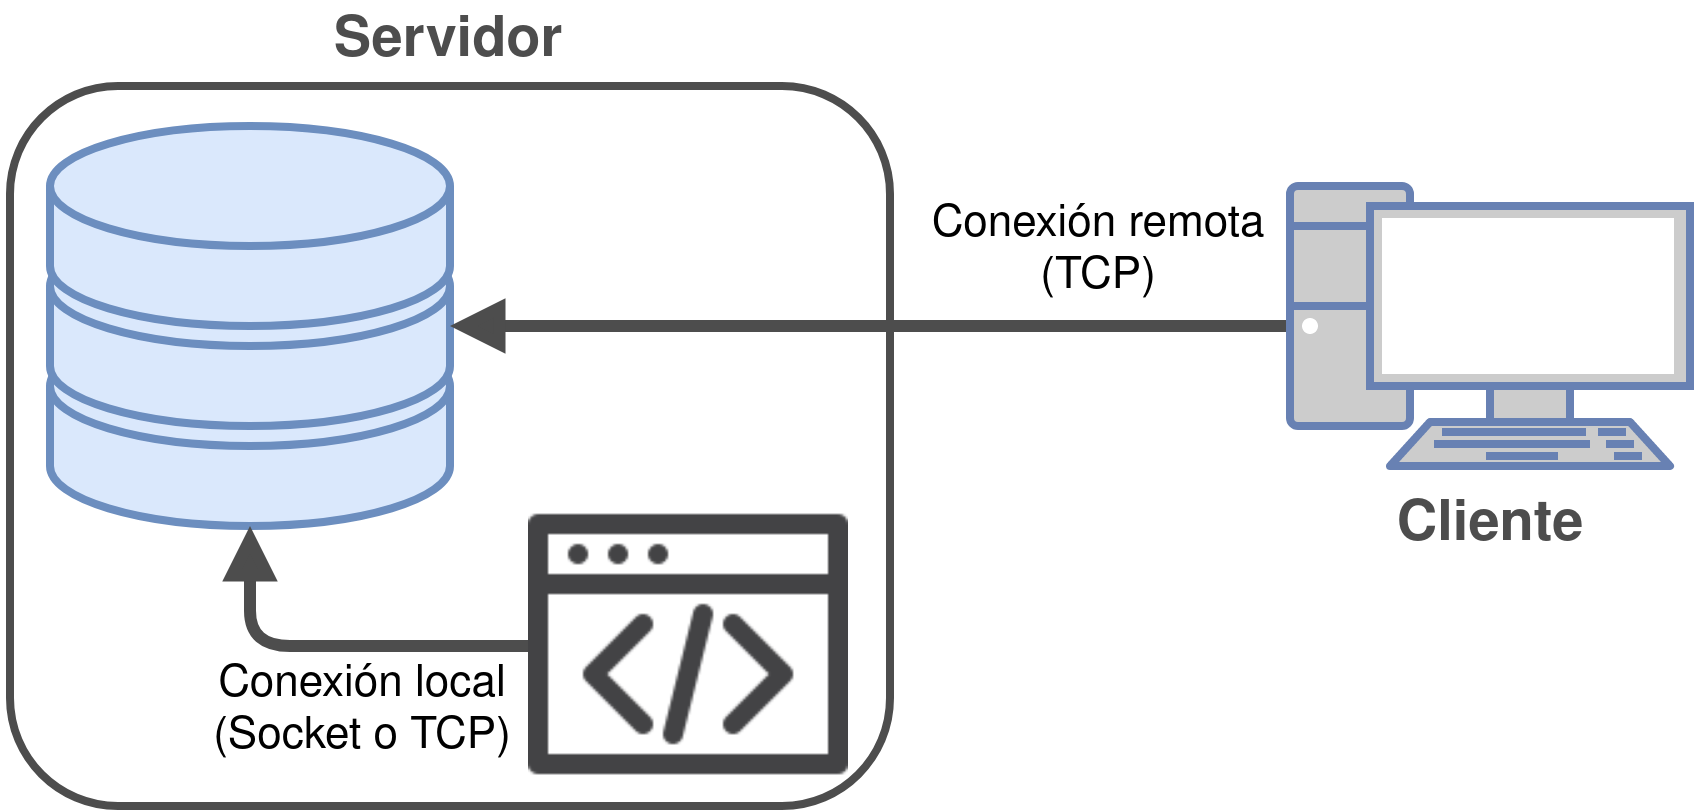
\includegraphics[width=0.6\linewidth]{cliente_servidor.png}
\end{center}

El cliente que efectúa la conexión puede encontrarse en la misma máquina donde está situado el servidor (conexión local) o desde una máquina externa (conexión remota).


\subsection{Conexión local (Socket)}
En entornos UNIX existe la posibilidad de realizar la conexión a ciertos servidores que están en la misma máquina desde la que se origina la conexión, mediante lo que se denomina un \textbf{Unix domain Socket}.

\textbf{Los sockets} en entornos GNU/Linux se pueden ver como un fichero, y \textbf{son un medio de comunicación entre procesos que se ejecutan en la misma máquina}.

La configuración estándar de MySQL arranca creando un fichero Socket en la siguiente ruta por defecto \configfile{/var/run/mysqld/mysqld.sock}, por lo que la posibilidad de realizar una conexión local mediante dicho socket es posible.

De hecho, nada más realizar la instalación de MySQL es la única manera de poder realizar la conexión y sólo será posible desde el usuario root:

\begin{center}
    \vspace{-15pt}
    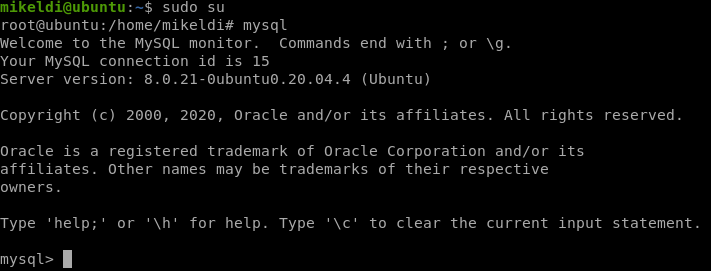
\includegraphics[width=0.8\linewidth]{console_1.png}
    \vspace{-20pt}
\end{center}

Como se puede ver, en la imagen, los pasos para poder realizar la conexión han sido:
\begin{enumerate}
    \item Convertirnos en root
    \item Ejecutar el comando    \commandbox{mysql}.
\end{enumerate}

Este comando es el \textbf{Cliente} MySQL que realizará la conexión contra el Servidor MySQL. Debido a que no se le ha pasado ningún parámetro al comando, éste realizará un primer intento de conexión a la ruta del socket estándar (indicada anteriormente).

Una vez realizada la conexión veremos que nos aparece un \textit{prompt}  \inlineconsole{mysql>} que indica que la conexión se ha realizado correctamente y estamos en el CLI (\textit{Command Line Interface}, Interfaz de Línea de Comandos) donde podremos ejecutar órdenes de configuración, administración o peticiones a las bases de datos.

